%! Author = teismar
%! Date = 5/19/24
%! File = main.tex

% Preamble
\documentclass[
    11pt,
    ngerman,
    toc=listof,
    toc=bibliography
]{scrartcl}

%! Author = teismar
%! Date = 5/19/24
%! File = Preamble.tex

% Packages
% Add this near the beginning of your preamble, after other package includes
% \usepackage[utf8]{inputenc} % not needed with LuaLaTeX
\usepackage{graphicx}        % Include images
\usepackage{setspace}      % Allows setting line spacing
\usepackage{textcomp}        % Additional symbols
\usepackage{ifthen}          % Conditional statements
\usepackage{pgffor}           % For-loops
\usepackage[a4paper, left=4cm, right=2cm, top=2.5cm, bottom=2cm]{geometry} % Page layout
\usepackage{fontspec}        % Font selection (for LuaTeX and XeTeX)
\usepackage{scrlayer-scrpage} % This package is similar to fancyhdr
\usepackage[ngerman]{babel}  % This line enables German language support
\usepackage{csquotes} 
\usepackage{hyperref}       % Hyperlinks
\usepackage{microtype}       % Improve general typography
\usepackage{pgfplots}        % Create plots directly in LaTeX
\usepackage{xcolor}          % Color support
\usepackage{amsmath}         % Math support
\usepackage{booktabs}        % Better tables
\usepackage{float}           % Better control over float positions
\usepackage{csvsimple}       % Read CSV files
\usepackage{listings}        % Code listings
\usepackage{etoc}           % Extensive ToC handling
\usepackage{dirtree}         % Directory trees
\usepackage{dirtytalk}      % Quotes
\usepackage{tcolorbox}      %Color Box
\usepackage{tikz}
\usetikzlibrary{shapes, arrows, positioning, fit}

\pgfplotsset{compat=1.17}    % Set the pgfplots compatibility version

% KOMA-Script
\KOMAoptions{listof=totoc}  % Include List of Figures/Tables in the ToC
\KOMAoptions{bibliography=totoc} % Include Bibliography in the ToC

% Font settings for LuaTeX
\setmainfont{Arial}

% Set 1.5 line spacing for the entire document    
\onehalfspacing    

% Hyperref
\hypersetup{
    colorlinks = true,          % Enable colored links
    urlcolor = blue,            % Color for external hyperlinks
    linkcolor = black,          % Color of internal links (set to black or document text color)
    citecolor = black           % Color of citations (set to black or document text color)
}

% Colors
\definecolor{telekommagenta}{HTML}{E20074}
\definecolor{darkgreen}{rgb}{0.0, 0.5, 0.0}

% Style
    % Clears all header and footer fields, equivalent to \fancyhf{}
    \clearpairofpagestyles

    % Header configurations
        \ihead{\leftmark}             % Displays the current section name in the header
        \ohead{\thepage}              % Displays the page number in the header

        % Set a line under the header
        \KOMAoptions{headsepline=true}

        % Automatically mark each section to update \leftmark
        \renewcommand{\sectionmark}[1]{\markboth{#1}{}}

        % Set up for no paragraph indentation and using the scrheadings style
        \setlength{\parindent}{0pt}
        \pagestyle{scrheadings}


% Bibliography
\usepackage[backend=biber, style=apa]{biblatex}
\addbibresource{main.bib}  % Add your .bib file here



% Listings
\usepackage{color}
\definecolor{codegreen}{rgb}{0,0.6,0}
\definecolor{codegray}{rgb}{0.5,0.5,0.5}
\definecolor{codepurple}{rgb}{0.58,0,0.82}
\definecolor{backcolour}{rgb}{0.95,0.95,0.92}

\lstdefinestyle{mystyle}{
    backgroundcolor=\color{backcolour},
    commentstyle=\color{codegreen},
    keywordstyle=\color{magenta},
    numberstyle=\tiny\color{codegray},
    stringstyle=\color{codepurple},
    basicstyle=\ttfamily\footnotesize,
    breakatwhitespace=false,
    breaklines=true,
    captionpos=b,
    keepspaces=true,
    numbers=left,
    numbersep=5pt,
    showspaces=false,
    showstringspaces=false,
    showtabs=false,
    tabsize=2
}

\lstdefinestyle{termstyle}{
    backgroundcolor=\color{gray!10}, % light gray background
    basicstyle=\ttfamily\small,      % the size of the fonts that are used for the code
    breakatwhitespace=false,         % sets if automatic breaks should only happen at whitespace
    breaklines=true,                 % sets automatic line breaking
    captionpos=b,                    % sets the caption-position to bottom
    keepspaces=true,                 % keeps spaces in text, useful for keeping indentation of code (possibly needs columns=flexible)
    numbers=none,                    % where to put the line-numbers; possible values are (none, left, right)
    numberstyle=\tiny\color{gray},   % the style that is used for the line-numbers
    showspaces=false,                % show spaces everywhere adding particular underscores; it overrides 'showstringspaces'
    showstringspaces=false,          % underline spaces within strings only
    showtabs=false,                  % show tabs within strings adding particular underscores
    tabsize=2,                       % sets default tabsize to 2 spaces
    frame=single,                    % adds a frame around the code
    rulecolor=\color{black},         % if not set, the frame-color may be changed on line-breaks within not-black text (e.g. comments (green here))
    escapeinside={\%*}{*)},          % if you want to add LaTeX within your code
    morekeywords={*,...},            % if you want to add more keywords to the set
}


\lstset{style=mystyle}

%! Author = Tim Eismar
%! Date = 5/19/24

\newcommand{\pruefung}{Bachelorarbeit}
\newcommand{\titlePruefung}{Dies ist ein supertolles Thema}
\newcommand{\abgabeTermin}{04.02.1969}
\newcommand{\abgabeOrt}{Hannover}
\newcommand{\modul}{ModulXY}
\newcommand{\pruefer}{Prof. Dr. Johann Sünde}
\newcommand{\insitution}{Leibniz-Fachhochschule}
\newcommand{\insitutionLogo}{images/LeibnizFH-Logo}

\newcommand{\authorName}{Dieter Müller}
\newcommand{\matrikelnummer}{12345}

\newcommand{\includeBetrieb}{true}
\newcommand{\betriebLogo}{images/Telekom-Logo}
\newcommand{\betriebName}{Deutsche Telekom AG}
\newcommand{\betriebAnschift}{Bonner Talweg 100}
\newcommand{\betriebOrt}{53113 Bonn}

\newcommand{\studiengang}{IT-Security}
\newcommand{\jahrgang}{2022}


% Formatting
\newcommand{\br}[1][1]{%
    \foreach \n in {1,...,#1} {%
        \bigbreak
    }%
}

% Abkürzungen, ggfs. mit korrektem Leerraum
\newcommand{\eur}[1]{\mbox{#1\,\texteuro}\xspace}
\newcommand{\ua}{\mbox{u.\,a.}\xspace}
\newcommand{\zB}{\mbox{z.\,B.}\xspace}

% verschiedene Befehle um Wörter semantisch auszuzeichnen ----------------------
\newcommand{\Index}[2][\empty]{\ifthenelse{\equal{#1}{\empty}}{\index{#2}#2}{\index{#1}#2}}
\newcommand{\Fachbegriff}[2][\empty]{\ifthenelse{\equal{#1}{\empty}}{\textit{\Index{#2}}}{\textit{\Index[#1]{#2}}}}
\newcommand{\NeuerBegriff}[2][\empty]{\ifthenelse{\equal{#1}{\empty}}{\textbf{\Index{#2}}}{\textbf{\Index[#1]{#2}}}}

\newcommand{\Ausgabe}[1]{\texttt{#1}}
\newcommand{\Eingabe}[1]{\texttt{#1}}
\newcommand{\Code}[1]{\texttt{#1}}
\newcommand{\Datei}[1]{\texttt{#1}}

\newcommand{\Assembly}[1]{\textsf{#1}}
\newcommand{\Klasse}[1]{\textsf{#1}}
\newcommand{\Methode}[1]{\textsf{#1}}
\newcommand{\Attribut}[1]{\textsf{#1}}

\newcommand{\Datentyp}[1]{\textsf{#1}}
\newcommand{\XMLElement}[1]{\textsf{#1}}
\newcommand{\Webservice}[1]{\textsf{#1}}

\newcommand{\Refactoring}[1]{\Fachbegriff{#1}}
\newcommand{\CodeSmell}[1]{\Fachbegriff{#1}}
\newcommand{\Metrik}[1]{\Fachbegriff{#1}}
\newcommand{\DesignPattern}[1]{\Fachbegriff{#1}}



% Document
\begin{document}
    %! Author = teismar
%! Date = 5/19/24

\begin{titlepage}
    \begin{center}
        % FH Logo
        \expandafter\includegraphics\expandafter[width=0.4\textwidth]{\insitutionLogo} % Adjusted logo size for better proportion
        \vspace{1cm} % Space between logo and title

        % Title
        {\LARGE \pruefung\\[0.5cm]}
        {\Huge\textbf{\titlePruefung}}\\

        \vspace{2cm} % Space between title and author

        % Author
        {\huge \authorName}\\
        \vspace{2cm} % Space between author and institution

        % Additional Details in Tabular form
        \large{
        \begin{tabular}{ll}
        Matrikelnummer: & \matrikelnummer\\
        Studiengang: & \studiengang\\
        Jahrgang: & \jahrgang\\
        Modul: & \modul\\
        Prüfer: & \pruefer\\
        Abgabetermin: & \abgabeTermin\\
        Institution: & \insitution\\
        \end{tabular}
        }
        \vspace{2cm} % Adjusted space for a balanced look

        % Conditional inclusion of Employer Logo and Address
        \ifthenelse{\equal{\includeBetrieb}{true}}{%
            % Title
            {\Large \textbf{Arbeitgeber:}}\\
            \vspace{0.5cm}
            % Employer Logo
            \expandafter\includegraphics\expandafter[height=2cm]{\betriebLogo}\\
            % Employer Address
            \large \betriebName\\
            \normalsize \betriebAnschift\\
            \normalsize \betriebOrt\\
            \vspace{1cm}
        }{}


        % Date
        {\large \today} % Automatically adds today's date


        \vfill % Pushes the following text to the bottom of the page


    \end{center}
\end{titlepage}

    % Sperrvermerk ----------------------------------------------------------------
    \section*{Sperrvermerk}
\label{sec:Sperrvermerk}
Diese Arbeit enthält vertrauliche Informationen der \betriebName, insbesondere in Bezug auf \titlePruefung. Die darin enthaltenen Interviews sowie die Analyse der internen Strukturen und Prozesse unterliegen der Vertraulichkeit.
\br
Die vorliegende Arbeit darf ohne ausdrückliche Genehmigung des Autors \textbf{und} der \betriebName weder ganz noch teilweise veröffentlicht oder Dritten zugänglich gemacht werden. Eine Einsichtnahme ist lediglich den Prüfern der \insitution sowie den durch den Verfasser und die Deutsche Telekom AG autorisierten Personen gestattet. Eine Vervielfältigung oder Weitergabe der Arbeit, auch in Auszügen, ist ohne Zustimmung des Autors \textbf{und} der \betriebName  untersagt.
\br
Die Vertraulichkeit der Interviews und der darin enthaltenen Aussagen ist zu jeder Zeit zu wahren.


    % ToC -------------------------------------------------------------------------

    \renewcommand{\contentsname}{Inhaltsverzeichnis}
    \tableofcontents
    \cleardoublepage


    % Inhalt ---------------------------------------------------------------------
    %! Author = teismar
%! Date = 5/19/24
%! File = Inhalt.tex

%! Author = teismar
%! Date = 9/17/24
%! File = Einfuerung.tex

\section{Einführung}
\label{sec:Einfuehrung}

In dieser Arbeit wird ein Konzept zur Entwicklung eines Systems vorgestellt, das die Erkennung von Anomalien in Zeitreihen ermöglicht. Das System soll in der Lage sein, sowohl bekannte als auch unbekannte Anomalien zu identifizieren und dabei eine hohe Genauigkeit und Robustheit aufzuweisen. Ziel ist es, ein Werkzeug zu schaffen, das in verschiedenen Anwendungsbereichen eingesetzt werden kann, um frühzeitig auf potenzielle Probleme aufmerksam zu machen und somit präventive Maßnahmen zu ermöglichen. \autocite{Neumann2024Jan}

%! Author = teismar
%! Date = 9/17/24
%! File = Grundcharakter.tex
\cleardoublepage
\section{Kapitel 2}
\label{sec:kap2}

Hier ist ein weiteres Beispiel für eine Tabelle, die den Vergleich zwischen traditionellen und flexiblen Unternehmensmodellen verdeutlicht. Diese Tabelle zeigt die Unterschiede in Struktur, Entscheidungsfindung, Kommunikation, Arbeitsteilung, Mitarbeiterrolle, Fokus sowie Stärken und Schwächen der beiden Modelle.
\begin{table}[H]
    \centering
    \caption{Vergleich traditioneller und flexibler Unternehmensmodelle}
    \label{tab:vergleich_modelle}
    \begin{tabular}{|p{4cm}|p{5cm}|p{5cm}|}
        \hline
        \textbf{Merkmal} & \textbf{Traditionelles Modell} & \textbf{Flexibles Modell} \\ \hline
        Struktur & Hierarchisch, starr & Flach, anpassungsfähig \\ \hline
        Entscheidungsfindung & Top-down & Dezentral, teamorientiert \\ \hline
        Kommunikation & Formal, vertikal & Offen, horizontal \\ \hline
        Arbeitsteilung & Streng, spezialisiert & Flexibel, teamübergreifend \\ \hline
        Mitarbeiterrolle & Ausführend & Mitgestaltend, eigenverantwortlich \\ \hline
        Fokus & Effizienz, Stabilität & Agilität, Innovation \\ \hline
        Stärken & Klare Verantwortlichkeiten, Stabilität in vorhersehbaren Umgebungen & Anpassungsfähigkeit, Innovationskraft, Mitarbeiterzufriedenheit \\ \hline
        Schwächen & Starrheit, langsame Entscheidungsfindung, geringe Mitarbeitermotivation & Hoher Koordinationsbedarf, erfordert hohe Eigenverantwortung der Mitarbeiter \\ \hline
    \end{tabular}
\end{table}
%! Author = teismar
%! Date = 9/17/24
%! File = TradToSpot.tex
\cleardoublepage
\section{Spotify-Modell}
\label{sec:Spoitfy}

\begin{figure}[H]
    \centering % Centers the image within the figure environment.
    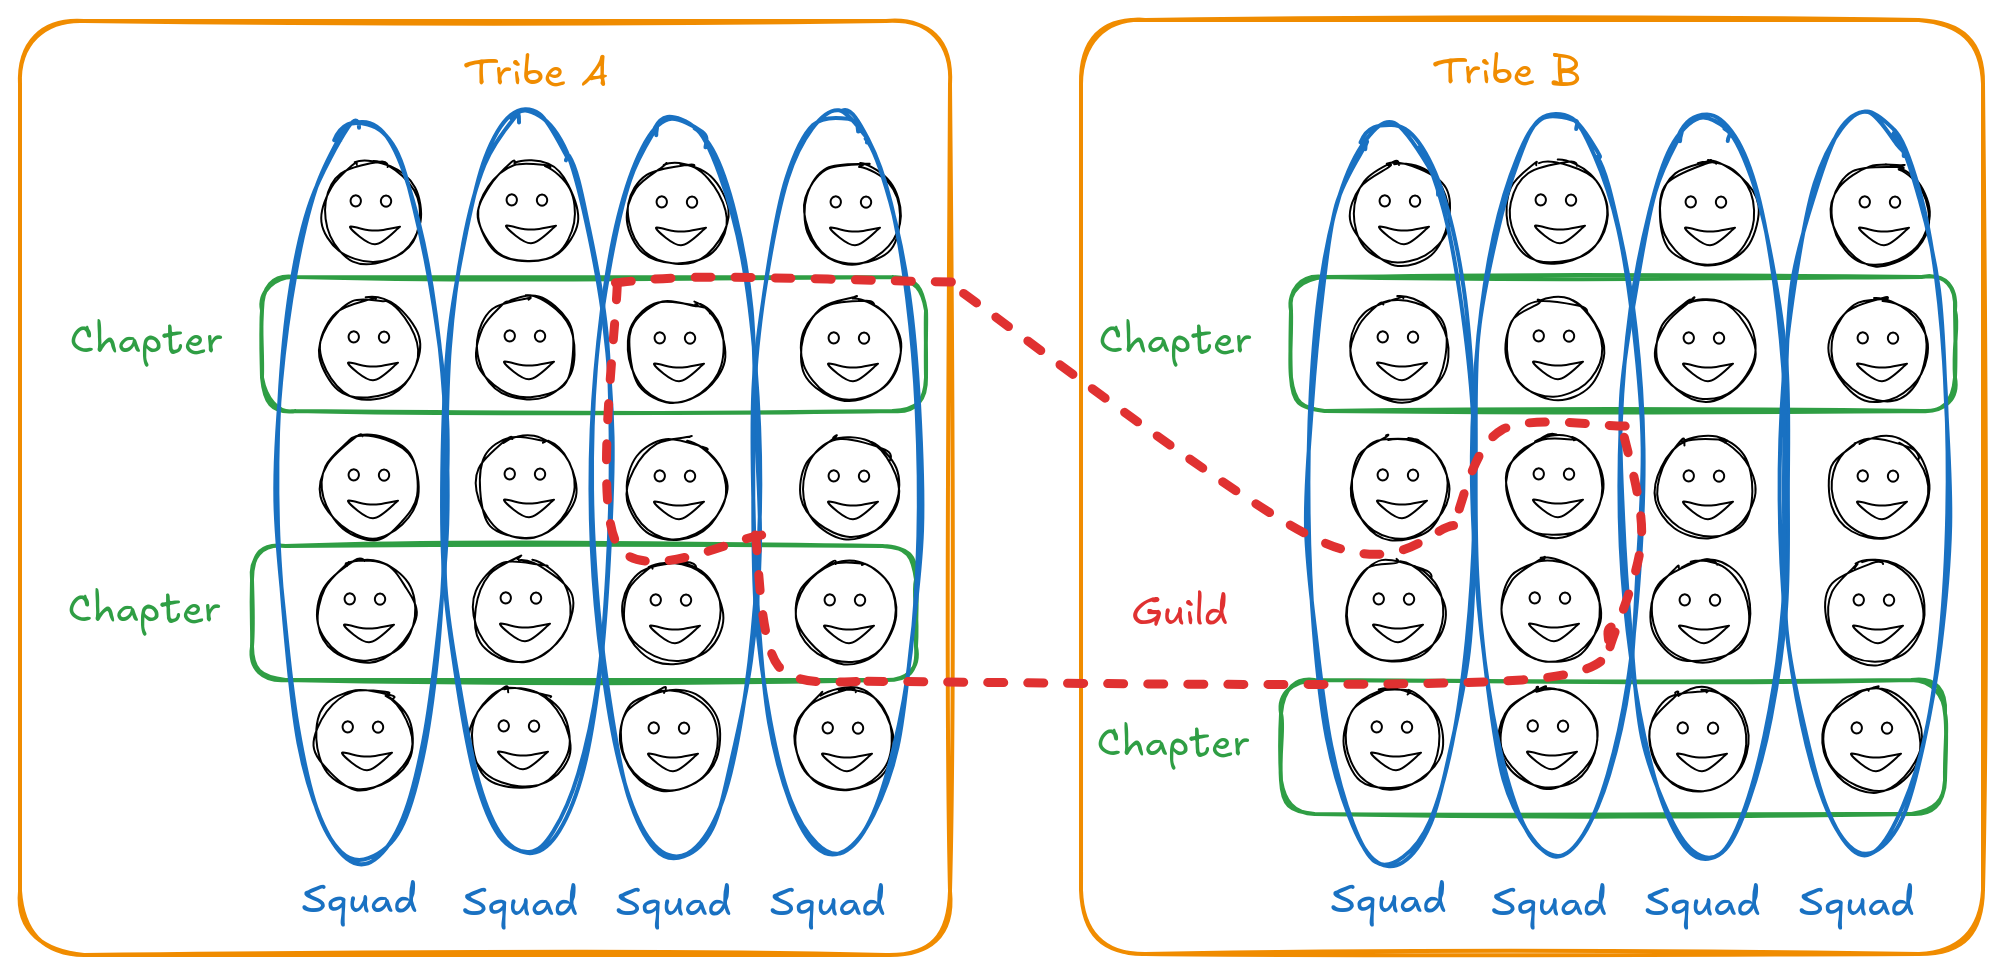
\includegraphics[width=\textwidth]{images/spot} % Include the image with a certain scaling.
    \caption{Das Spotify-Modell: Eine Grafik zur Veranschaulichung der Struktur und Prinzipien. | Eigendarstellung}
    \label{fig:spotify_model} % Add a label to refer to the image.
\end{figure}


%! Author = teismar
%! Date = 9/17/24
%! File = Praxisfall.tex
\cleardoublepage
\section{Praxisfall}
\label{sec:Praxisfall}

In der Praxis bin ich von der Klippe gestoßen worden. Ich habe mich mit dem Thema \textit{Künstliche Intelligenz} beschäftigt und bin auf die Frage
\begin{quote}
    \textit{Wie kann ich meine eigene KI erstellen?}
\end{quote}

%! Author = teismar
%! Date = 9/17/24
%! File = Fazit.tex
\cleardoublepage
\section{Fazit}
\label{sec:Fazit}


Lorem ipsum dolor sit amet, consectetur adipiscing elit. Donec a diam lectus. Sed sit amet ipsum mauris. Maecenas congue ligula ac quam viverra nec consectetur ante hendrerit. Donec et mollis dolor. Praesent et diam eget libero egestas faucibus et in libero. Suspendisse potenti. Nunc feugiat mi a tellus consequat imperdiet.
    \listoftables
    \cleardoublepage
    \listoffigures
    \cleardoublepage

    % Literatur ------------------------------------------------------------------
    \clearpage
    \renewcommand{\refname}{Literaturverzeichnis}
    \printbibliography[title={Literaturverzeichnis}]

    % Erklärung ------------------------------------------------------------------
    \clearpage
    \addsec{Selbstständigkeitserklärung}

Hiermit erkläre ich, \authorName, dass ich die vorliegende Arbeit selbstständig und ohne fremde Hilfe
verfasst und keine anderen Hilfsmittel als die angegebenen verwendet habe.
\br
Insbesondere versichere ich, dass ich alle wörtlichen und sinngemäßen Übernahmen
aus anderen Werken – dazu gehören auch Internetquellen – als solche kenntlich
gemacht habe.
\br[5]

\abgabeOrt, den \today \hspace{0.05cm}
\rule[-0.2cm]{6cm}{0.5pt}
\textsc{\authorName}

    % Anhang ---------------------------------------------------------------------
    \clearpage
    %! Author = teismar
%! Date = 5/19/24
%! File = Anhang.tex


\appendix
\pagenumbering{Roman}  % Römische Seitenzahlen
\section{Anhang}
\label{appendix:Anhang}

\subsection{Interview mit Santa Claus, Wünscherfüller}

\textbf{Frage: Wie lange wurde der Bart nicht rasiert?} \\
\textbf{Antwort:} Locker ne Woche

\subsection{Website Snapshots}
\begin{tcolorbox}[colframe=telekommagenta, colback=white, coltitle=black, title=Personal Webiste of Tim Eismar, sharp corners]
    \begin{itemize}
        \item \textbf{Source:} \href{https://teismar.de}{\textcolor{telekommagenta}{Homepage - Tim Eismar}}
        \item \textbf{Date:} \textit{20.09.2024, 1:11:20AM}
        \item \textbf{File:} \texttt{KeyElementsOfSpotifyAgileScalingModel.png} (appended)
    \end{itemize}
\end{tcolorbox}

\dirtree{%
.1 Appendix.
.2 SnapshotHomepageTeismar.png.
}
\end{document}
